\subsubsection*{Training Insights}
Training the VGG19 model was not very different from the VGG16 model. It also struggled to predict values above a mass of $\log{(M_{500}^{\text{true}}/M_{\odot})} \sim 14.3$ and the predictions are widely spread throughout the mass range. Even the best model did not produce useful predictions for galaxy mass estimations.


\subsubsection*{Best Performing Model}
The best performing VGG19 model did not perform very well. Its results are very similar to the ones from the best performing VGG16 model with similar $\sigma$ and $\mu$ values on both the test and training set.

\begin{figure}[h]
\centering
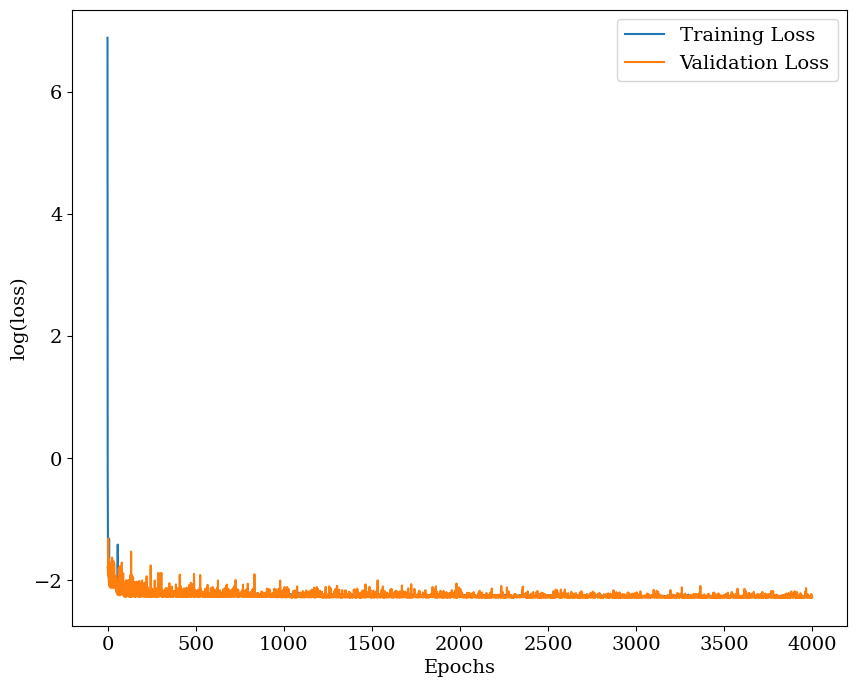
\includegraphics[width=.667\textwidth]{images/Chapter4/VGG19/vgg19_history.png}
\caption{As with VGG16, VGG19 is not able to learn in any way. Training and validation loss are close to each other throughout the whole training, indicating no overfitting but also no improvement in accuracy. } 
\label{fig:vgg19_best_history}
\end{figure}


Over all ten trainings, VGG19 was not able to give accurate predictions on neither the test nor the training set. As mentioned in \cref{vgg_16_res}, I do not know the core of this problem. It is possible though, that the model struggles to find any useful filters in training the convolutions, so that it is not able to detect any features. All it learned then was how to spread the galaxy clusters evenly to achieve the best possible loss without recognizing any galaxy cluster features. This would explain why the model only predicts values between $\log{(M_{500}^{\text{true}}/M_{\odot})} = 13.4$ and $\log{(M_{500}^{\text{true}}/M_{\odot})} = 14.4$, because the most clusters are within this mass range (see \autoref{fig:data_dist}).
All in all, VGG models seem to be difficult to train with galaxy cluster data and optimization would be needed to get useful results. A smaller learning rate could help to avoid the brought up issues.


\begin{figure}[H]
\centering
\begin{subfigure}{.46\textwidth}
  \centering
  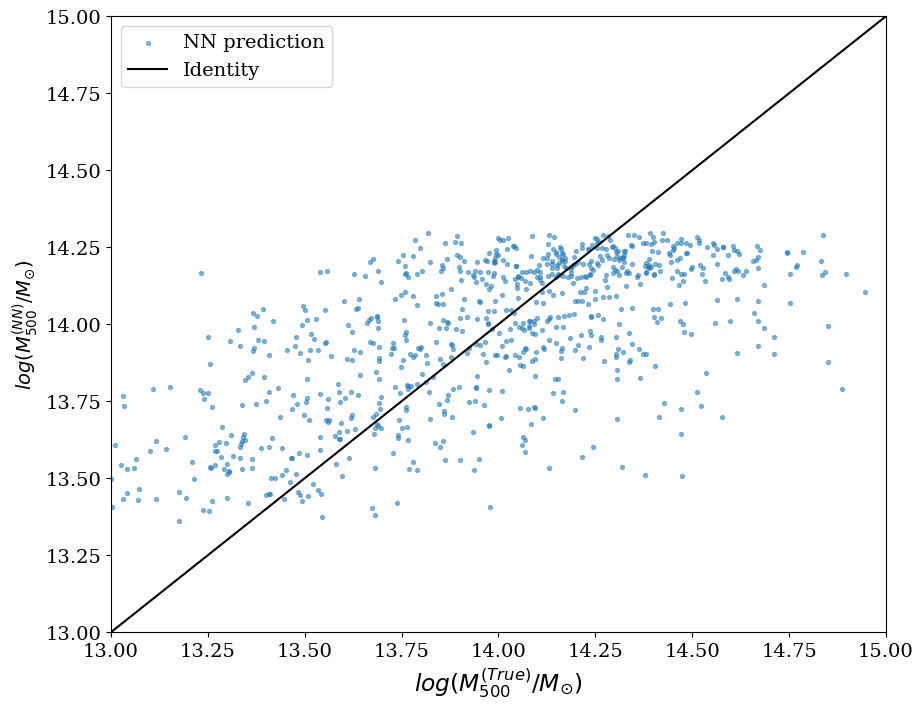
\includegraphics[width=\linewidth]{images/Chapter4/VGG19/vgg19_test.png}
  \caption{Model predictions on the test set.}
  \label{fig:best_perf_vgg19_a}
\end{subfigure}%
\hspace{.6em}
\begin{subfigure}{.46\textwidth}
  \centering
  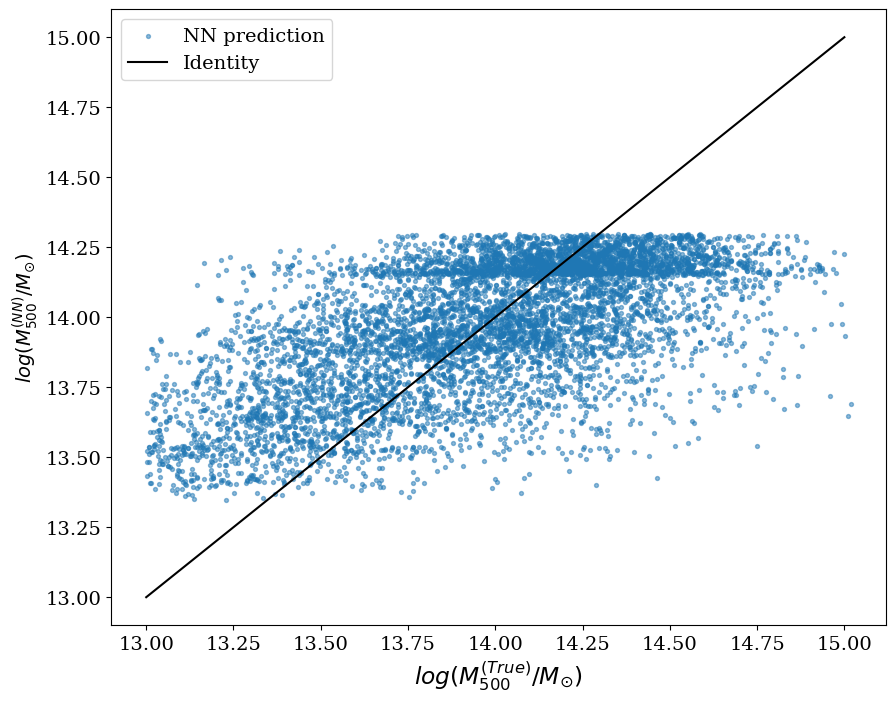
\includegraphics[width=\linewidth]{images/Chapter4/VGG19/vgg19_train.png}
  \caption{Model predictions on the training set.}
  \label{fig:best_perf_vgg19_b}
\end{subfigure}
\begin{subfigure}{.46\textwidth}
  \centering
  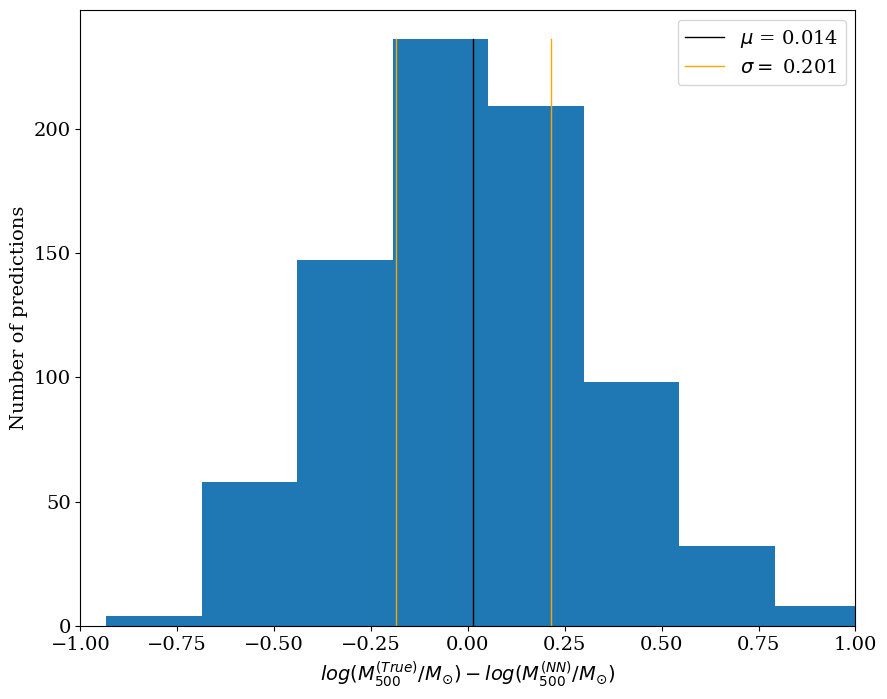
\includegraphics[width=\linewidth]{images/Chapter4/VGG19/vgg19_test_hist.png}
  \caption{Histogram of model predictions on the test set.}
  \label{fig:best_perf_vgg19_c}
\end{subfigure}%
\hspace{.6em}
\begin{subfigure}{.46\textwidth}
  \centering
  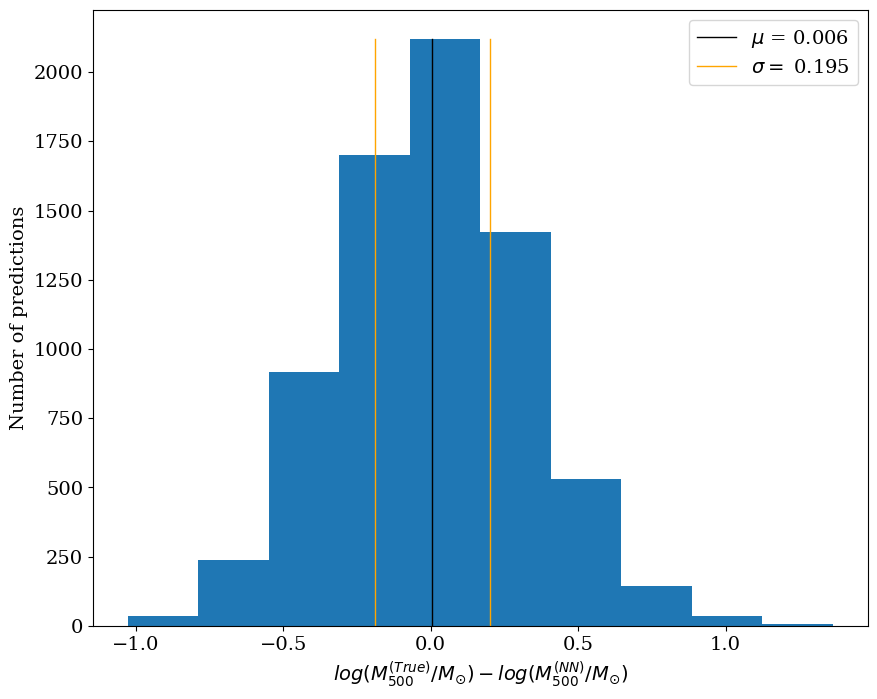
\includegraphics[width=\linewidth]{images/Chapter4/VGG19/vgg19_train_hist.png}
  \caption{Histogram of model predictions on the training set.}
  \label{fig:best_perf_vgg19_d}
\end{subfigure}
\caption{VGG19 is not able to predict accurately even on the training set. The results look similar to the predictions from VGG16} 
\label{fig:best_perf_vgg19}
\end{figure}

